\documentclass[10pt, compress]{beamer}

\usetheme[titleprogressbar]{m}

\usepackage{booktabs}
\usepackage[scale=2]{ccicons}
\usepackage{minted}

\usepgfplotslibrary{dateplot}

\usemintedstyle{trac}

\title{Kernel Methods}
\subtitle{}
\date{\today}
\author{Chih-Wei Chang \and Chung-Yen Hung}
\institute{Department of Mathematics, National Taiwan University}

\begin{document}

\maketitle

\section{Introduction}

\begin{frame}[fragile]
  \frametitle{Motivation}

  \begin{block}{Linear Model}
    \begin{enumerate}
      \item Simple and Well Studied
      \item Computationally Feasible
    \end{enumerate}
  \end{block}

  \begin{block}{Real-world Problems}
    \begin{enumerate}
      \item Non Linear
      \item Sophisticated Interdependencies
    \end{enumerate}
  \end{block}

  \begin{description}
    \item[Question] Can we apply \textbf{Linear Model} on \textbf{Real-world Problems}?
  \end{description}

\end{frame}

\begin{frame}[fragile]
  \frametitle{Motivation Cont.}

  \begin{block}{How about \textbf{Feature Transform}?}
    Mapping features to higher dimensional space. For example, the quadratic transformation from \(\mathbb{R}^2\) to \(\mathbb{R}^6\)
    \[
      \Phi: (x_1, x_2) \mapsto (x_1^2, x_2^2, \sqrt{2} x_1 x_2, \sqrt{2} x_1, \sqrt{2} x_2, 1).
    \]

    Line in \(\mathbb{R}^6\) corresponds to quadratic curve in \(\mathbb{R}^2\).
    Common techniques in the machine learning world.

    \begin{description}[<+- | alert@+>]
      \item[Learning Stage] Fit linear model \(h: \mathbb{R}^6 \rightarrow \{0, 1\} \) on \(\Phi(\mathbf{x})\).
      \item[Testing Stage] \(h(\Phi(\mathbf{x}_{test}))\) gives the prediction.
    \end{description}

  \end{block}

\end{frame}

\begin{frame}[fragile]{Motivation Cont.}

  However \dots
  \begin{description}[<+- | alert@+>]
    \item[Pros] Fitting complicated underlying rules -- the higher the dimension, the more powerful the model.
    \item[Cons] Extra computational costs, e.g., inner products -- the higher the dimension, the harder the computation.
  \end{description}
\end{frame}


\begin{frame}[fragile]{Kernel Trick}

  Luckily, \textbf{Kernel Trick} comes to rescue \dots
  \begin{enumerate}[<+- | alert@+>]
    \item Mathematical shortcut for preventing computing inner product directly.
    \item Combine the favors of Linearity and Non-Linearity.
  \end{enumerate}
\end{frame}

\begin{frame}[fragile]{Kernel Trick Cont.}

  \begin{block}{Kernel Trick}
    Consider the inner product in the previous example
    \begin{align*}
      \langle \Phi(\mathbf{x}), \Phi(\mathbf{y}) \rangle &= {\Phi(\mathbf{x})}^T \Phi(\mathbf{y}) \\
          &= x_1^2 y_1^2 + x_2^2 y_2^2 + 2 x_1 x_2 y_1 y_2 + 2 x_1 y_1 + 2 x_2 y_2 + 1 \\
          &= {(\mathbf{x}^T\mathbf{y} + 1)}^2 = {(\langle \mathbf{x}, \mathbf{y} \rangle + 1)}^2
    \end{align*}

    It implies we can define a special function
    \[
      K(\mathbf{x}_1, \mathbf{x_2}) = \langle \Phi(\mathbf{x_1}), \Phi(\mathbf{x_2}) \rangle,
    \]
    which is the so-called kernel function.

  \end{block}

\end{frame}

\section{Common Kernel}

\begin{frame}[fragile]{Polynomial Kernel}

  \begin{block}{Polynomial Kernel}

    Suppose we use the polynomial feature transformation \( \Phi_{d}(x) \), which collects all the possible coefficients in the \(d\)-degree polynomial.

    We then have the polynomial kernel
    \[
      K_{\Phi_{d}}(x, y) = {(\langle x,y \rangle + \alpha)}^{d}
    \]
  \end{block}

\end{frame}

\begin{frame}[fragile]{Polynomial Kernel Cont.}

  \begin{block}{Quadratic Transformation as An Special Case}
    Let \( d=2 \), the transformation
    \begin{align*}
      \Phi_{2}(x) =& (x_{n}^{2}, \dots, x_{1}^{2}, \sqrt{2}x_{n}x_{n-1}, \dots, \sqrt{2}x_{n}x_{1}, \sqrt{2}x_{n-1}x_{n-2}, \dots, \\
                  &\sqrt{2c}x_{n}, \dots, \sqrt{2c}x_{1}, c)
    \end{align*}
    And the kernel function
    \begin{align*}
    K(x, y) &= (\sum_{i=1}^{n} x_{i}y_{i} + c)^{2} \\
      &= \sum_{i=1}^{n}x_{i}^{2}y_{i}^{2} + \sum_{i=2}^{n}\sum_{j=1}^{i-1}(\sqrt{2}x_{i}x_{j})(\sqrt{2}y_{i}y_{j}) + \sum_{i=1}^{n}(\sqrt{2c}x_{i})(\sqrt{2c}y_{i}) + c^{2}
    \end{align*}
  \end{block}
\end{frame}


\begin{frame}[fragile]{Gaussian Kernel}

  \begin{block}{Gaussian Kernel}
    The Gaussian Kernel is defined as
    \[
      K(x, y) = \exp(-\gamma{\| x-y \|}^{2}), \text{with \( \gamma > 0\)}
    \]
  \end{block}

\end{frame}

\begin{frame}[fragile]{Gaussian Kernel Cont.}
  \begin{block}{As An Extreme Case of Polynomial Kernel}
    For \(\gamma = 1\)
    \begin{equation}
      \begin{split}
          K(x, y) &= \exp({\| x-y \|}^{2}) \\
                  &= \exp(-{x}^{2})\exp(-{y}^{2})\exp({2xy}) \\
                  &= \exp(-{x}^{2})\exp(-{y}^{2})(\sum_{i=0}^{\infty}\frac{{(2xy)}^{i}}{i!}) \\
                  &= \sum_{i=0}^{\infty}(\exp(-{x}^{2}\sqrt\frac{2^{i}}{i!}){x}^{i})(\exp(-{y}^{2}\sqrt\frac{2^{i}}{i!}){y}^{i}) \\
                  &= \Phi{(x)}^{T}\Phi(y)\\
      \end{split}
    \end{equation}
    It implies \(\Phi(x) = \exp(-{(x)}^{2})(1, \sqrt\frac{2}{1!}x, \sqrt\frac{2^{2}}{2!}x^{2}, \dots)\).
  \end{block}
\end{frame}

\section{Kernel Machines}

\begin{frame}[fragile]{Kernel SVM}
  \begin{block}{Soft Margin SVM dual}
    \[
      \max_{\forall \alpha \geq 0, \forall \beta \geq 0}\big(\min_{b, w} \frac{1}{2}{w}^{T}w + C\sum_{n=1}^{N}{\xi}_{n} + \sum_{n=1}^{N} {\alpha}_{n}(1-{\xi}_{n}-{y}_{n}({w}^{T}{z}_{n} + b)) + \sum_{n=1}^{N}{\beta}_{n}(-\xi)\big)
    \]
    by KKT condition
    \[
      \max_{\forall 0 \leq \alpha \leq C, {\beta}_{n} = C-\alpha_{n}} -\frac{1}{2}\sum_{n=1}^{N}{||{\alpha}_{n}y_{n}x_{n}||}^{2} + \sum_{n=1}^{N}{\alpha}_{n}
    \]
  \end{block}
\end{frame}

\begin{frame}[fragile]{Kernel SVM Cont.}
  \begin{block}{Soft Margin SVM dual}
    Unfold formula and multiply -1.
    \[
      \min_{\alpha} \frac{1}{2}\sum_{n=1}^{N}\sum_{m=1}^{N}{\alpha}_{n}{\alpha}_{m}y_{n}y_{m}{\color{red}{x_{n}}^{T}x_{m}} - \sum_{n=1}^{N}{\alpha}_{n}
    \]

    \[
      \text{subject to  } \sum_{n=1}^{N}y_n{\alpha}_{n} = 0 \text{; } {\alpha}_{n} \geq 0 \text{, } \forall n \in [0,N] \text{, } n \in \mathbb{N}
    \]

    \[
      \text{implicitly  } w =\sum_{n=1}^{N}{\alpha}_{n}y_{n}x_{n} \text{; } {\beta}_{n} = C - \alpha_{n} \text{, } \forall n \in [0,N] \text{, } n \in \mathbb{N}
    \]
    We can do kernel method on red side \({\color{red}{x_{n}}^{T}x_{m}}\)

  \end{block}
\end{frame}

\begin{frame}[fragile]{Kernel SVM Cont.}
  \begin{block}{Example: Linear SVM}
    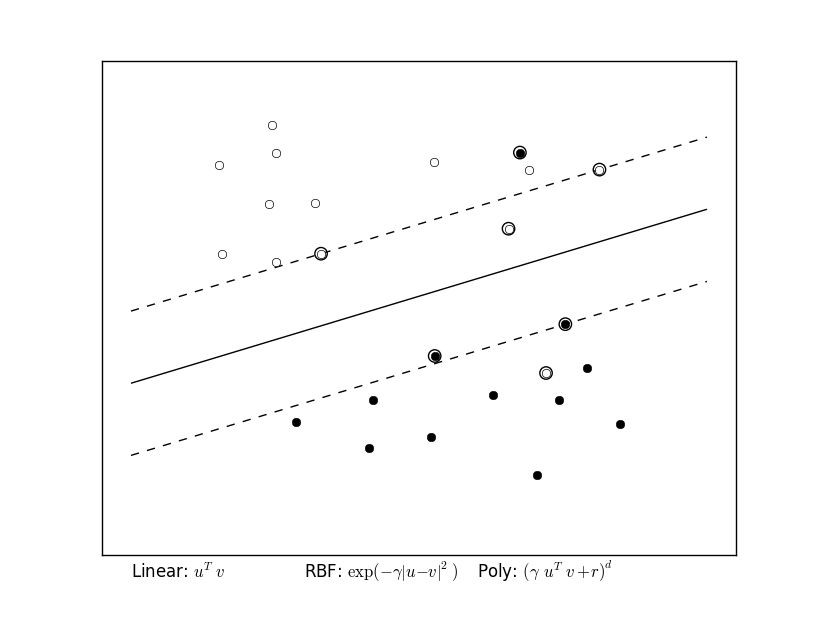
\includegraphics[width=\textwidth, height=.7\textheight]{images/linear.png}
  \end{block}
\end{frame}

\begin{frame}[fragile]{Kernel SVM Cont.}
  \begin{block}{Example: Degree 2 Poly Kernel SVM}
    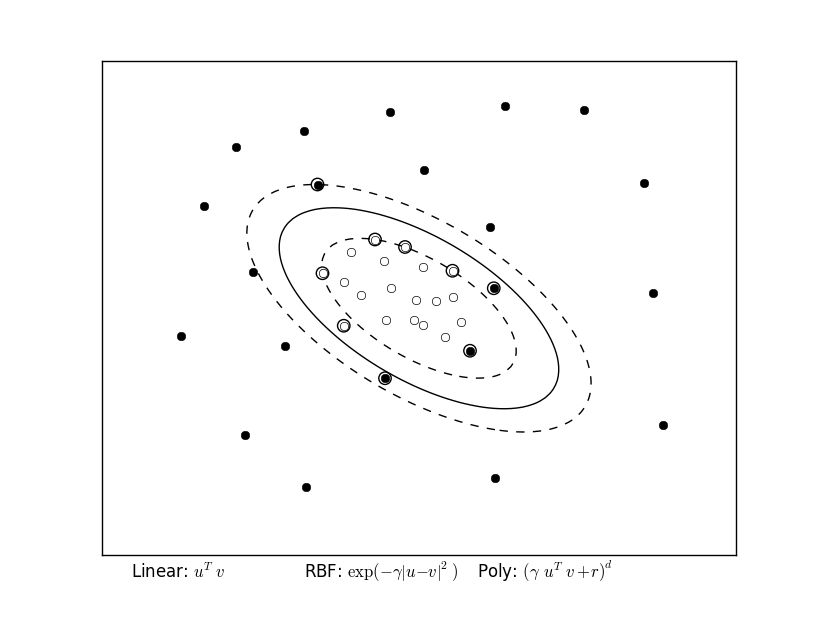
\includegraphics[width=\textwidth, height=.7\textheight]{images/quadratic.png}
  \end{block}
\end{frame}

\begin{frame}[fragile]{Kernel SVM Cont.}
  \begin{block}{Example: Gaussian Kernel SVM}
    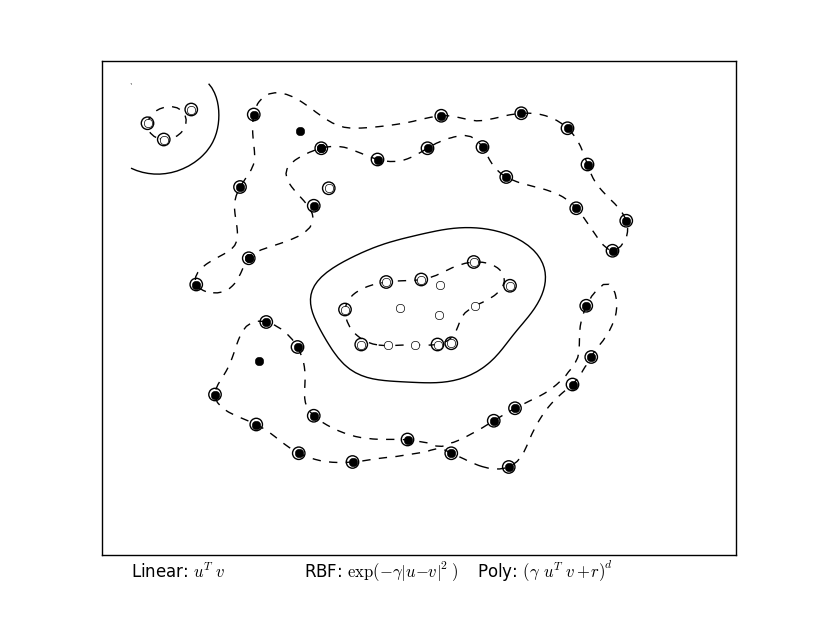
\includegraphics[width=\textwidth, height=.7\textheight]{images/non_linear.png}
  \end{block}
\end{frame}


\begin{frame}[fragile]{Kernel Ridge Regression}
  \begin{block}{Ridge Regression}
    Minimize the quadratic cost as well as the regularization term
    \[
      C(\mathbf{w}) = \frac{1}{2} \sum_{i} {(y_i - \mathbf{w}^T\mathbf{x}_i)}^2 + \frac{1}{2} \lambda {\| \mathbf{w} \|}^2
    \]

    We have analytic solution
    \[
      \mathbf{w} = {(\lambda \mathbf{I} + \sum_{i} \mathbf{x}_i \mathbf{x}_i^T )}^{-1} (\sum_{j} y_j \mathbf{x}_j)
    \]
  \end{block}
\end{frame}

\begin{frame}[fragile]{Kernel Ridge Regression Cont.}
  \begin{block}{Plug the Kernel Function In}
    Note that
    \[
      {(P^{-1} + B^T R^{-1} B)}^{-1} B^T R^{-1} = PB^T {(BPB^T + R)}^{-1}
    \]

    Therefore,
    \begin{align*}
      \mathbf{w} &= {(\lambda \mathbf{I} + \sum_{i} \phi(\mathbf{x}_i) {\phi(\mathbf{x}_i)}^T )}^{-1} (\sum_{j} y_j \phi(\mathbf{x}_j)) \\
                &= {(\lambda \mathbf{I} + \Phi \Phi^T) }^{-1} \Phi \mathbf{y} \\
                &= \Phi {(\Phi^T \Phi + \lambda I)}^{-1} \mathbf{y}
    \end{align*}
  \end{block}
\end{frame}

\begin{frame}[fragile]{Kernel Ridge Regression Cont.}
  \begin{block}{Prediction}
    In the prediction stage, we first transform \( \phi(\mathbf{x}_{test}) \)
    \[
      y = \mathbf{w}^T \phi(\mathbf{x}_{test}) = \mathbf{y}^T {(\Phi^T \Phi + \lambda I)}^{-T} {\Phi}^T \phi(\mathbf{x}_{test})
    \]

    All the calculation can be done in terms of inner product, and hence we can apply the kernel trick.
  \end{block}
\end{frame}

\begin{frame}[fragile]{Example: Kernel PCA v.s. PCA}
  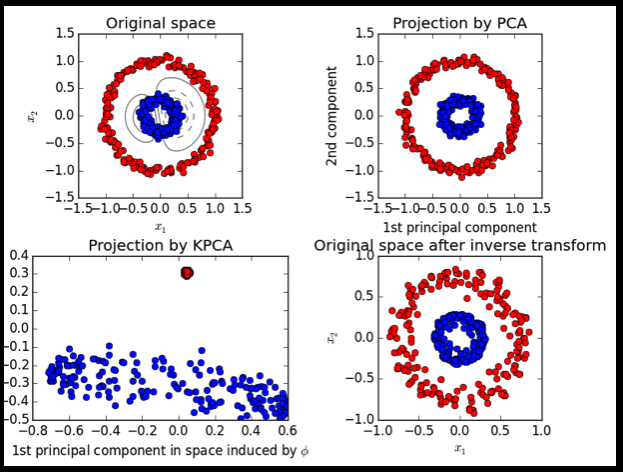
\includegraphics[width=\textwidth, height=.7\textheight]{images/KPCA.png}
\end{frame}

\begin{frame}[fragile]{Example: PCA of IRIS dataset}
  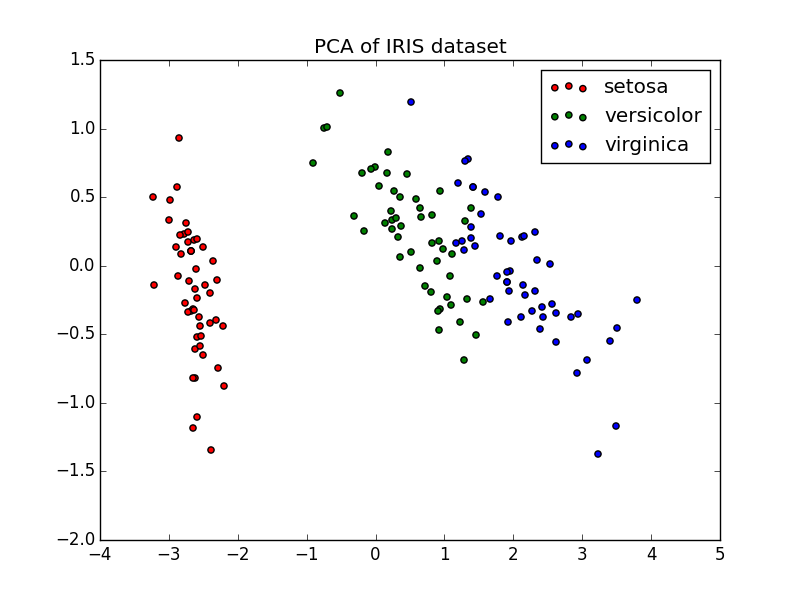
\includegraphics[width=\textwidth, height=.7\textheight]{images/iris_pca.png}
\end{frame}

\begin{frame}[fragile]{Example: Kernel PCA of IRIS dataset}
  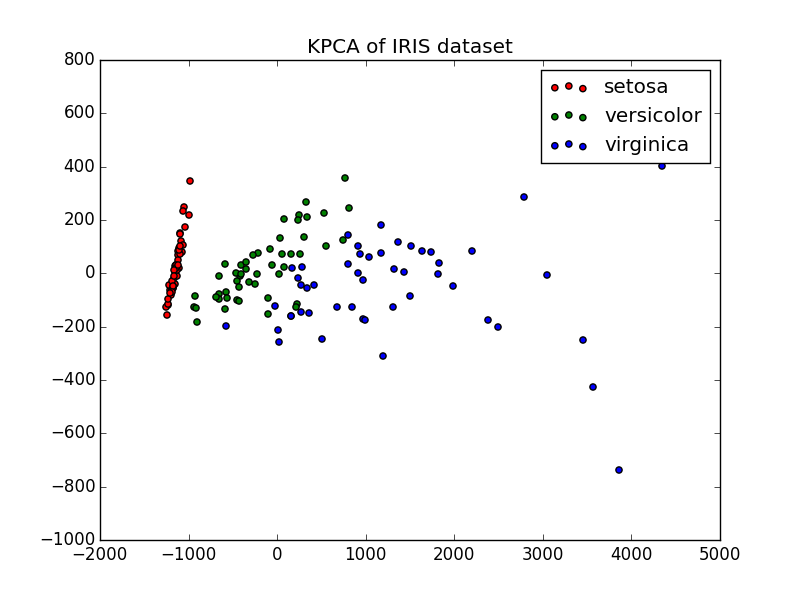
\includegraphics[width=\textwidth, height=.7\textheight]{images/iris_kpca.png}
\end{frame}

\begin{frame}[fragile]{Example: PCA of PENDIGITS dataset}
  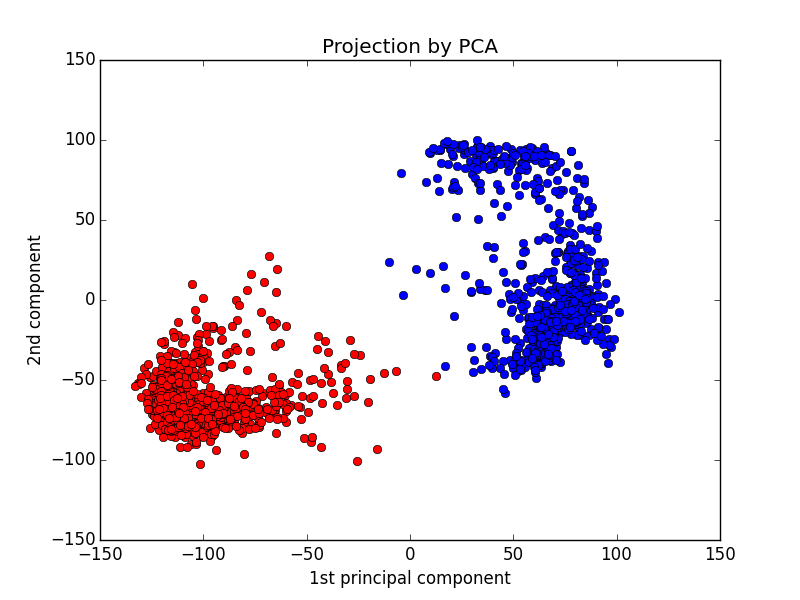
\includegraphics[width=\textwidth, height=.7\textheight]{images/pca_pen.png}
\end{frame}

\begin{frame}[fragile]{Example: Kernel PCA of PENDIGITS dataset}
  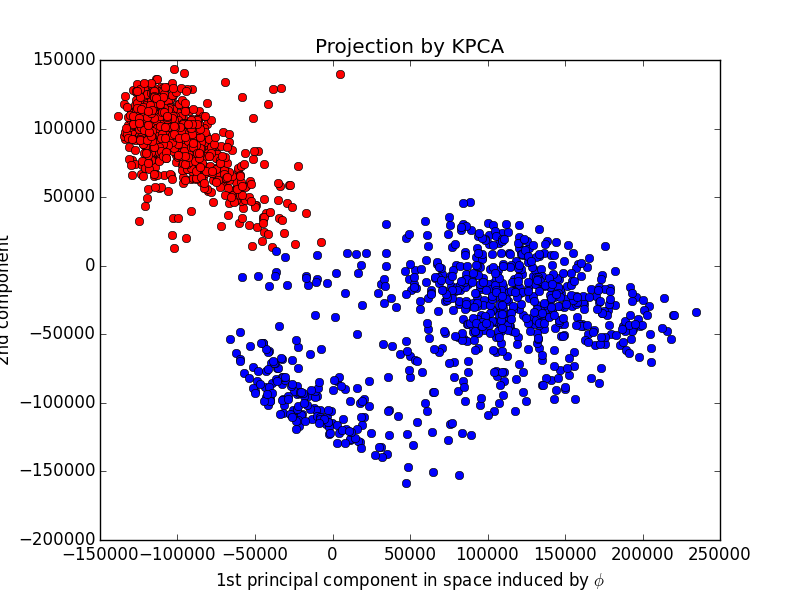
\includegraphics[width=\textwidth, height=.7\textheight]{images/kpca_pen.png}
\end{frame}
\section{Conclusion}

\begin{frame}{Summary}

  \begin{itemize}
    \item Linear to Non-linear
    \item Computationally Feasible
    \item Ability to Fit Arbitrarily Complicated Model
  \end{itemize}

\end{frame}

\plain{Questions?}

\end{document}
